\documentclass[border=2mm]{standalone}
\usepackage{tikz}
\begin{document}
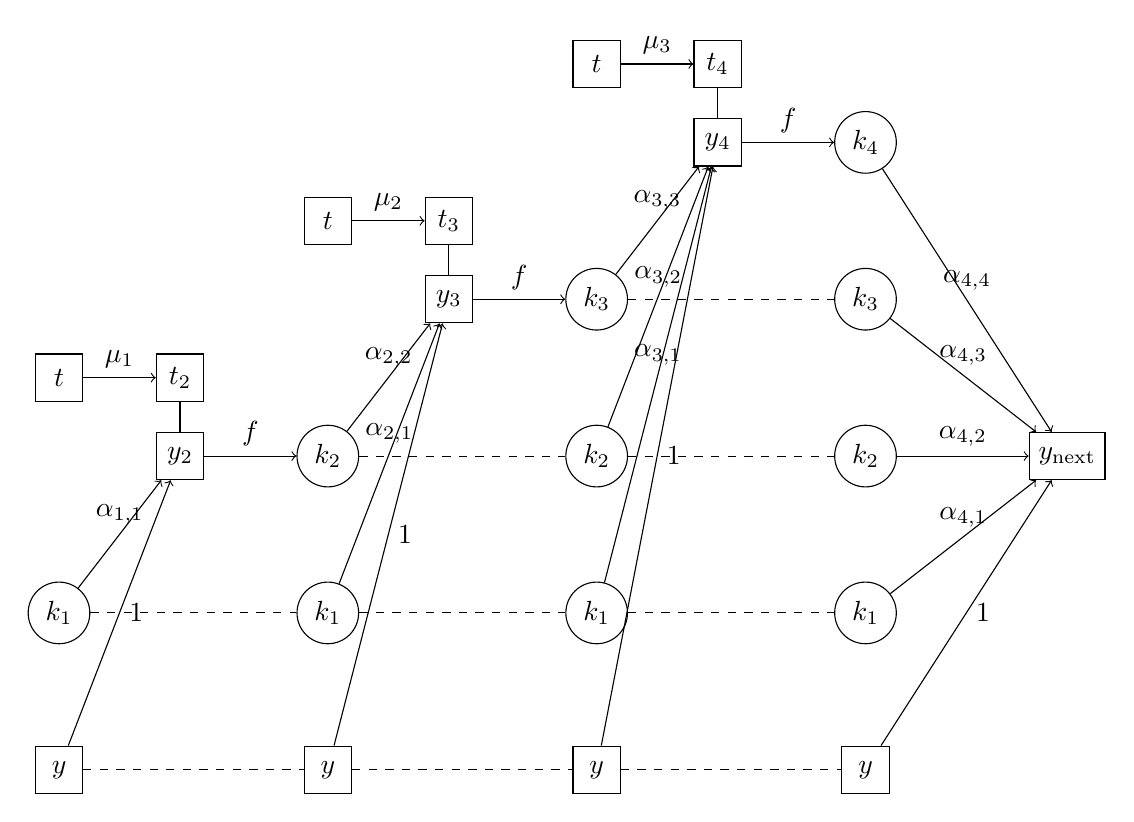
\begin{tikzpicture}
% Constants
\def\circleRadius{0.4cm} % Radius of the circles
\def\squareRadius{0.6cm} % Radius of the circles
\def\columnSpacing{0.12cm} % Horizontal spacing between columns
\def\rowSpacing{0.07cm} % Vertical spacing between rows
\def\leftShift{-2cm} % Shift to the left

% Draw the circles in a triangular formation
\foreach \col in {2, 3, 4, 5} {
    \foreach \row in {1,...,\col} {
        % Calculate the x and y positions
        \pgfmathsetmacro\x{\leftShift + (\col-1)*\columnSpacing}
        \pgfmathsetmacro\y{(\row-1)*\rowSpacing}
        % Draw the circle with labels
        \ifnum\row=1
            \node[rectangle, draw, minimum size=\squareRadius] (circle-\col-\row) at (\x, \y) {$y$};
        \else
            \node[circle, draw, minimum size=\circleRadius] (circle-\col-\row) at (\x, \y) {$k_{\number\numexpr\row-1\relax}$};
        \fi
    }
}

% Draw squares and connect to next column's circle
\foreach \col in {2, 3, 4} {
    % Calculate the x and y positions for the square
    \pgfmathsetmacro\xSquare{\leftShift + (\col-0.55)*\columnSpacing}
    \pgfmathsetmacro\ySquare{\col*\rowSpacing}
    \pgfmathsetmacro\xtSquare{\leftShift + (\col-1)*\columnSpacing}
    \pgfmathsetmacro\ytSquare{(\col+0.5)*\rowSpacing}
    \pgfmathsetmacro\nextcol{int(\col + 1)}
    \node[rectangle, draw, minimum size=\squareRadius] (square-\col) at (\xSquare, \ySquare) {$y_\col$};
    \node[rectangle, draw, minimum size=\squareRadius] (squaret0-\col) at (\xtSquare, \ytSquare) {$t$};
    \node[rectangle, draw, minimum size=\squareRadius] (squaret-\col) at (\xSquare, \ytSquare) {$t_\col$};
    % Store the node names in variables
    \edef\fromnode{square-\col}
    \edef\tonode{circle-\nextcol-\nextcol}
    % Draw arrow using the stored node names with f annotation
    \draw[->] (\fromnode) -- node[above] {$f$} (\tonode);
    % Draw arrow with μ_(col-1) annotation
    \pgfmathsetmacro\prevcol{int(\col-1)}
    \draw[->] (squaret0-\col) -- node[above] {$\mu_{\prevcol}$} (squaret-\col);
    \draw[-] (squaret-\col) -- (\fromnode);
}

% Draw horizontal dashed lines between circles at the same height
\foreach \row in {1,...,5} {
    \foreach [remember=\col as \prevcol (initially 2)] \col in {3,...,5} {
        \ifnum\row<\col
            \draw[dashed] (circle-\prevcol-\row) -- (circle-\col-\row);
        \fi
    }
}

% Connect circles to squares with horizontal arrows and modified alpha annotations
\foreach \col in {2, 3, 4} {
    \foreach \row in {1,...,\col} {
        % Calculate previous indices
        \pgfmathsetmacro\prevcol{int(\col-1)}
        \pgfmathsetmacro\prevrow{int(\row-1)}
        % Draw horizontal arrow from circle to square with modified alpha annotation
        \ifnum\row=1
            \draw[->] (circle-\col-\row) -- node[right] {$1$} (square-\col);
        \else
            \draw[->] (circle-\col-\row) -- node[above] {$\alpha_{\prevcol,\prevrow}$} (square-\col);
        \fi
    }
}

% Add the additional column with y_next
\pgfmathsetmacro\xNext{\leftShift + 4.75*\columnSpacing}
\pgfmathsetmacro\yNext{2*\rowSpacing}
\node[rectangle, draw, minimum size=\squareRadius] (y-next) at (\xNext, \yNext) {$y_{\rm next}$};

% Add arrows from the second-to-last column (column 4) to y_next
\foreach \row in {1,...,5} {
    \ifnum\row=1
        \draw[->] (circle-5-\row) -- node[right] {$1$} (y-next);
    \else
        \draw[->] (circle-5-\row) -- node[above] {$\alpha_{4,\number\numexpr\row-1\relax}$} (y-next);
    \fi
}

\end{tikzpicture}
\end{document}